\documentclass[tikz, margin=3.14mm]{standalone}
\usepackage{amsmath, amsfonts, amssymb}
\usepackage{mathtools}
\usepackage{mathrsfs}
\usetikzlibrary{arrows.meta, positioning}

\begin{document}
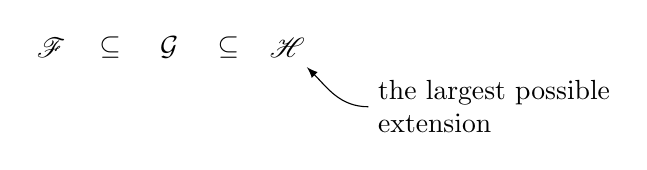
\begin{tikzpicture}[scale=1.5]
\node at (0,0) {$\mathscr F$};
\node at (0.5, 0) {$\subseteq$};
\node at (1,0) {$\mathcal G$};
\node at (1.5, 0) {$\subseteq$};
\node (h) at (2, 0) {$\mathscr H$}; 
\node (text) [align=left] at (3.75, -.5) {the largest possible\\extension};

\draw [-latex] (text.west) to [in=-45, out=180] (h);

\end{tikzpicture}
\end{document}